
\chapter{Aufbau und Analyse der ETL Prozesse}

\section{Wettervorhersagen}

Wettervorhersagen haben das Ziel den Zustand der Erdatmosphäre zu
einer bestimmten Zeit an einem bestimmten Ort zu prognostizieren. Sie
werden meist von staatlichen oder privaten Wetterdiensten erstellt,
die sich an den Erkenntnissen der Meteorologie bedienen. Heutige
Wettervorhersagen basieren auf den aufwendig berechneten Ergebnissen
numerischer Wettermodelle.

Die Vorhersage des Wetters ist ein Anfangswertproblem, das meist in
drei Schritten gelöst wird. Im ersten Schritt, der Analyse, wird der
Ausgangszustand der Atmosphäre bestimmt. Dieser Zustand wird durch
verschiedene physikalische Größen festgelegt, die von Wetterstationen,
Satelliten, Bojen oder Flugzeugen gemessenen werden. Typische Größen
repräsentieren dabei Luftdruck, Temperatur, Wind, Wasserdampf, Wolken
und Niederschlag.

Die Modellberechnung ist der zweite Schritt, und simuliert die
Entwicklung der Atmosphäre in die Zukunft. Die Berechnung dieser
Simulation ist sehr aufwendig, weshalb meist Supercomputer eingesetzt
werden. Ergebnis der Modellberechnung ist der Zustand der Atmosphäre
zu verschiedenen Zeitpunkten in der Zukunft, dargestellt durch
physikalischen Größen.

Im letzten Schritt, der Nachbereitung, werden die Ergebnisse der
Simulation schließlich für die verschiedensten Nutzer
aufbereitet. Dies beinhaltet die Generierung von Wetterkarten,
Warnhinweisen für Technisches Hilfswerk und Feuerwehr oder die
Visualisierung von Strömungsfilmen.

\subsection{Numerische Wettermodelle}

Numerische Wettermodelle versuchen den Zustand der Erdatmosphäre und
deren Veränderung im Laufe der Zeit als mathematisches Problem zu
beschreiben. Dabei werden die physikalischen Größen und Beziehungen,
die den Zustand und die Veränderung der Atmosphäre beschreiben, als
System partieller Differentialgleichungen modelliert. Die meisten
Modelle verwenden dabei dieselben physikalischen Gesetzmäßigkeiten,
die auf den Erhaltungssätzen von Energie, Impuls und Masse
beruhen. Meist unterscheiden sie sich aber in der konkreten
mathematischen Formulierung und der numerischen Lösung der
Gleichungssysteme, weshalb die Ergebnisse verschiedener Modelle
voneinander abweichen können.

\subsubsection{Operative Wettermodelle}

Der Deutsche Wetterdienst betreibt drei verschiedene
Wettermodelle. Die lokalen \textit{COSMO-DE} und \textit{COSMO-EU}
Modelle liefern Vorhersagen für Deutschland und Europa, das globale
Modell \textit{GME} hingegen Vorhersagen für die ganze Welt. Weitere
bekannte Modelle sind das von der US-amerikanischen \textit{National
  Oceanic and Atmospheric Administration} betriebene \textit{Global
  Forecast System (GFS)} \nomenclature{GFS}{Global Forecast System}
und das neuere \textit{Weather Research and Forecasting (WRF)}
\nomenclature{WRF}{Weather Research and Forecasting} Modell, das vom
\textit{National Weather Service (NWS)} \nomenclature{NWS}{National
  Weather Service}, vom amerikanischen Militär und einigen privaten
meteorologischen Organisationen verwendet wird.

\subsubsection{Diskretisierung von Raum und Zeit}

Um die sich verändernde Atmosphäre der Erde auf ein Modell abbilden zu
können wird eine Diskretisierung von Raum und Zeit vorgenommen. Dabei
wird die Oberfläche der Erde mit einem aus Drei- oder Vierecken
bestehenden Gitternetz überzogen, und die Atmosphäre vertikal in
mehrere Luftschichten aufgeteilt. Damit wird die unendlich Zahl der
möglichen Vorhersagepunkte in der Atmosphäre auf die endliche Zahl der
so entstandenen Kreuzungspunkte reduziert. In Abbildung
\ref{gitternetz} ist das dreieckige Gitternetz des zur Zeit vom
Deutschen Wetterdienst und des Max-Planck-Instituts für Meteorologie
neu entwickelten \textit{ICON} \nomenclature{ICON}{Icosahedral
  Non-hydrostatic General Circulation Model} Wettermodells zu sehen.

\begin{figure}[h]
  \begin{center}
    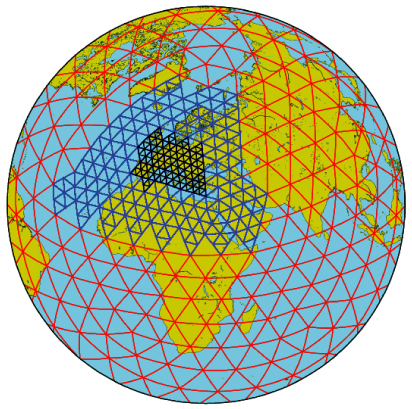
\includegraphics[height=200px]{bilder/gitternetz}
    \caption{Dreiecksgitter des ICON Wettermodells}
    \label{gitternetz}
  \end{center}
\end{figure}

Mit der Maschenweite bezeichnet man den horizontalen Abstand zwischen
zwei benachbarten Gitterpunkten. Je feiner das Gitter, bzw. je höher
die Auflösung des Modells ist, desto genauer kann die Erdoberfläche
und die darüber liegenden atmosphärischen Strukturen erfasst werden,
was sich auf die Genauigkeit der Wettervorhersage auswirkt. Die
benötigten Ressourcen zu Berechnung der Modellgleichungen steigt mit
der Anzahl der verwendeten Gitterpunkte.

Da eine sehr hohe Auflösungen selbst die Leistungsfähigkeit der
schnellsten Supercomputer übersteigt werden von den Wetterdiensten
meist verschiedene Modelle in unterschiedlichen Auflösungen
berechnet. Globale, den gesamten Globus umfassende Modelle werden mit
einer geringeren Auflösung als lokale, Länder oder Kontinente
abdeckende Modelle berechnet. Je weiter in die Zukunft prognostiziert
werden soll, desto mehr spielen aber wieder Wetterphänomene aus
Gebieten die nicht vom lokalen Modell abgedeckt werden eine Rolle. Für
Vorhersagen ab 5 Tagen in die Zukunft benötigen die lokalen Modelle
wiederum Informationen aus der gesamten Atmosphäre. Deshalb verwenden
die höher auflösenden lokalen Modelle oft Informationen als Randwerte
aus einem zuvor berechneten globalen Modell.

Die zeitliche Diskretisierung hingegen ist weniger problematisch. Die
meisten Modelle bieten mindestens Prognosen um 12 und 24 Uhr für
diejenigen Tage an, über die sich der Vorhersagezeitraum
erstreckt. Das \textit{Global Forecast System} Modell bietet
beispielsweise Vorhersagen im drei Stunden Intervall an, wobei das
lokale \textit{COSMO-DE} Modell mit einem 25 Sekunden Intervall
betrieben wird.

\subsubsection{Rechenaufwand heutiger Modelle}

In einer Präsentation
\footnote{\url{http://www.initiative-wissenschaftsjournalismus.de/fileadmin/Downloads/WissensWerte2008/B3_Majewski.pdf}}
aus dem November 2008 wurde der Rechenaufwand für die vom Deutschen
Wetterdienst betriebenen Modelle mit den dazugehörigen Kenngrößen
veröffentlicht. Damals wurden die Wettervorhersagen auf einem IBM
Power 5 System (p575) mit 52 Knoten, 416 Prozessoren und einer
Spitzenleistung von 3,1 Teraflop/s berechnet.

\begin{itemize}
\item Für Deutschland wird das \textit{COSMO-DE} Modell mit einer
  Maschenweite von 2,8 Kilometern betrieben und besteht aus ca. 10
  Millionen Gitterpunkten. Die Berechnung dauert 30 Minuten und
  liefert Vorhersagen in einem 25 Sekunden Intervall für einen
  21-stündigen Vorhersagezeitraum.
\item Das Europa umfassende Modell \textit{COSMO-EU} hat eine
  Maschenweite von 7 Kilometern, ca. 17 Millionen Gitterpunkten und
  wird mit einem Zeitintervall von 40 Sekunden erstellt. Die
  Berechnung einer 24-stündigen Vorhersage dauert 25 Minuten.
\item Das globale, die gesamte Welt umfassende \textit{GME} Modell hat
  eine Maschenweite von 40 Kilometern mit ca. 15 Millionen
  Gitterpunkten. Die Berechnung der 24 Stunden Vorhersage mit einem
  Zeitintervall von 133 Sekunden benötigt 15 Minuten.
\end{itemize}

Leider wurden während der Recherche keine genaueren Informationen
gefunden, wie sich die Berechnung der hier erwähnten Modelle auf dem
seit März 2009 beim Deutschen Wetterdienst in Betrieb genommenen
Vektorsupercomputer SX-9 der Firma NEC verhält. Die Spitzenleistung
dieses Systems beträgt momentan 4,5 Teraflop/s, die bis 2010 auf 11
Teraflop/s aufgestockt werden soll. Mit dieser neuen Anschaffung will
der Deutsche Wetterdienst unter anderem auch Wettervorhersagen mit
einer Auflösung von 2,8 Kilometern für Deutschlands Anrainerstaaten
berechnen.

\section{Überblick der verwendeten Datenquellen}

Eine der Anforderungen an die Web Applikation ist es den Nutzern
aktuelle Informationen über die Wetter- und die Wellenverhältnisse in
den nächsten Tagen zu bieten. Hierfür werden die frei erhältlichen
Ergebnisse von zwei numerischen Wettermodelle verwendet, dem
\textit{Global Forecast System} und dem \textit{Wave Watch III}
Modell.

\subsection{Global Forecast System}

Das \textit{Global Forecast System} ist ein globales numerisches
Wettermodell das vom \textit{National Weather Service} betrieben wird
und den gesamten Erdball abdeckt. Da die Ergebnisse der
Modellberechnung über das Internet
\footnote{\url{http://nomad5.ncep.noaa.gov/pub/gfs}} erhältlich sind
und von jedermann verwendet werden dürfen erfreut es sich einer großen
Beliebtheit. Das Modell liefert Vorhersagen bis zu 384 Stunden (16
Tage) in die Zukunft und wird mit variierenden Auflösungen viermal
täglich berechnet, jeweils um 0h, 6h, 12h und 18h koordinierter
Weltzeit (\textit{UTC}). Die ersten 180 Stunden werden mit einer
Maschenweite von ca. 40 Kilometern und einem Intervall von 3 Stunden
berechnet, die restlichen Stunden im 12 Stunden Intervall und einer
Auflösung von ca. 80 Kilometern. Vertikal wird die Atmosphäre bei
beiden Auflösungen in 64 unterschiedliche Luftschichten aufgeteilt.

Das Modell berechnet eine Vielzahl von physikalischen Größen, von
denen hier hauptsächlich die Temperatur, die Gesamtbewölkung und das
Niederschlagswasser von Bedeutung sind. Da weithin Einverständnis
darüber herrscht, dass Vorhersagen über 180 Stunden hinaus sehr
ungenau sind verwenden die hier entwickelten \textit{ETL} Prozessen
nur die ersten 180 Stunden in der höchsten verfügbaren Auflösung.

\subsection{Wave Watch III}

Um für mehr Sicherheit auf hoher See und an Küstenregionen zu sorgen
betreibt der \textit{National Weather Service} das \textit{Wave Watch
  III} Wettermodell um Wellen vorherzusagen. Es liefert ausschließlich
Informationen über diejenigen Wellen, die durch den direkten Einfluss
von Winden entstehen. Wellen die durch andere Ereignisse wie
z.B. Gewitter, Gezeiten oder Tsunamis verursacht werden, sind in
diesem Modell nicht berücksichtigt. Da sich Wellen viel zu sehr
voneinander unterscheiden, werden nicht Vorhersagen für einzelne
Wellen getroffen, sondern über die Statistik von mehreren Wellen. Das
Modell liefert sowohl Informationen über die Wellenhöhe, Wellenperiode
und Wellenrichtung als auch über die Windstärke und die Windrichtung
an einem bestimmten Ort zu einer bestimmten Zeit.

Das Modell wird wie das \textit{Global Forecast System} viermal
täglich neu berechnet, liefert Vorhersagen im 3 Stunden Intervall für
180 Stunden in die Zukunft und die Ergebnisse sind ebenfalls frei
erhältlich
\footnote{\url{http://polar.ncep.noaa.gov/waves/index2.shtml}}. Das
globale Modell wird mit einer Maschenweite von ca. 80 Kilometern
berechnet, die lokalen Modelle mit einer Maschenweite von bis zu 20
Kilometern. Die hier entwickelten \textit{ETL} Prozesse verarbeiten
bisher nur die Daten des globalen Modells.

\subsection{GRIB - Das GRIdded Binary Datenformat}

Die Abkürzung \textit{GRIB} \nomenclature{GRIB}{Gridded Binary} steht
für \textit{GRIdded Binary} und ist ein weit verbreitetes,
bitorientiertes Datenformat zur Speicherung und Übertragung von
Wetterdaten. Das Format wurde von der Kommision für Basissysteme
(\textit{CBS}) \nomenclature{CBS}{Commission for Basic Systems} der
Weltorganisation für Meteorologie (\textit{WMO})
\nomenclature{WMO}{World Meteorological Organization} standardisiert
\footnote{\url{http://www.wmo.int/pages/prog/www/WMOCodes/Guides/GRIB/GRIB1-Contents.html}}
und wird von vielen Wetterorganisationen dazu verwendet die Ergebnisse
ihrer Modellberechnungen kompakt und plattformunabhängig zu
speichern. Insgesamt wurden drei verschiedenen Versionen spezifiziert,
von denen sich die Versionen 1 und 2 etabliert haben. Die mit der
Nummer 0 bezeichnete Version wird als veraltet angesehen und befindet
sich bei den meisten Wetterorganisationen nicht mehr im operativen
Einsatz.

Eine \textit{GRIB} Datei besteht aus eigenständigen, sich selbst
beschreibenden Datensätzen, den sogenannten \textit{GRIB}
Nachrichten. Eine Nachricht enthält dabei alle Daten eines bestimmten
Produkts, für eine auf ein Gitternetz diskretisierte geographische
Region zu einem bestimmten Zeitpunkt. Beispielsweise die Temperaturen
um 12 Uhr mittags für Europa aus dem \textit{Global Forecast System},
oder die signifikanten Wellenhöhen des \textit{Wave Watch III} Modells
um 9 Uhr morgens für die gesamte Erdkugel. 

Eine \textit{GRIB} Nachricht besteht wiederum aus mehreren Sektionen,
die deren Inhalt genauer beschreiben und in Tabelle \ref{tab:grib}
aufgelistet sind. Die Sektionen enthalten neben den eigentlichen Daten
u.a. Informationen über die Dimension und Auflösung des verwendeten
Gitternetzes, die Herkunft der Daten, die Art des verwendeten
Komprimierungsverfahrens und die physikalische Einheit in der die
Daten gespeichert sind.

\begin{table*}
  \centering
  {\sf
    \footnotesize
    \begin{longtable}{@{}lp{10cm}@{}}

      \toprule
      \textbf{Name der Sektion} & \textbf{Verwendungszweck} \\

      \midrule

      Indicator & Die Zeichenkette ''GRIB'', Versionsnummer, Länge der gesamten Nachricht \\

      Identification & Charakteristiken die auf alle Daten zutreffen, u.a. Herkunft der Daten, Referenzzeit und Typ des Produkts \\

      Local Use (optional) & Abschnitt für beliebige zusätzliche Informationen \\

      Grid Definition &  Definition des Gitternetzes, u.a. die Dimension, die Anzahl der Datenpunkte und die verwendete Koordinatenprojektion \\

      Product Definition &  Beschreibung der Daten. \\

      Data Representation &  Beschreibung wie die Daten repräsentiert werden. Art der Komprimierung \\

      Bitmap & Eine Bitmap, welche die Anwesenheit bzw. Abwesenheit von Datenpunkten in der nächsten Sektion signalisiert \\

      Data &  Die komprimierten Daten. Für jeden in der Bitmap existierenden Gitterpunkt ein Wert. \\

      End & Die Zeichenkette ''7777'' markiert das Ende der Nachricht \\

      \bottomrule

    \end{longtable}
  }

  \caption{Die aufeinander folgenden Sektionen einer \textit{GRIB} Nachricht}
  \label{tab:grib}

\end{table*}

\textit{GRIB} Nachrichten können beliebig oft aneinandergereiht
werden, was eine individuelle Komposition von beliebigen Nachrichten
in einer Datei erlaubt. Dies wird in Abschnitt \ref{subsec:download}
ausgenutzt um nur ausgewählte Nachrichten einer größeren \textit{GRIB}
Datei zu beziehen.

\section{Datenbank Design}
\subsection{Konzeptionelle Schema}
\subsection{Physisches Schema}
\section{Extraktion aus den Quellsystemen}
\subsection{Download der GRIB Dateien}
\label{subsec:download}

\section{Transformation der Daten}
\section{Laden der Daten}
\section{Verbesserungen}

%%% Local Variables:
%%% mode: latex
%%% TeX-master: "../community-plattform"
%%% End:
